\documentclass{article}
\usepackage[margin=1in]{geometry}
\usepackage{enumerate,hyperref}
\usepackage{graphicx,listings}
\usepackage{xcolor}

\lstdefinestyle{sharpc}{language=[Sharp]C, frame=lr, rulecolor=\color{blue!80!black}}



\begin{document}
\lstset{style=sharpc}

\section{Graph Primitives}

\subsection{Graph}

A Graph object contains a list of vertices, a list of edges, and an adjacent list. Therefore, each vertex is implicitly assigned an id from 0 to n-1, each edge is implicitly assigned an id from 0 to m-1. For each vertex, the adjacency list contains the id of its neighbors.
 
\subsubsection{Read Graph From File: $O(m+n)$}
\begin{lstlisting}
String filename = "../../data/testgraph.txt";
Graph graph = GraphReader.Read(filename); 
\end{lstlisting}


\subsubsection{Insert a Vertex or an Edge: $O(1)$}
\begin{lstlisting}
Vertex vertex = new Vertex(vertexId);
graph.InsertVertex(vertex);
Edge edge = new Edge(node1Id, node2Id, edgeId);
graph.InsertEdge(edge);
\end{lstlisting}


\subsubsection{Deletion of a Vertex $v$: $O(d(v))$}
\begin{lstlisting}
graph.DeleteVertex(vertex);
\end{lstlisting}

\subsubsection{Deletion of an Edge: $O(1)$}
\begin{lstlisting}
graph.DeleteEdge(vertex1, vertex2);
\end{lstlisting}

\subsubsection{Iterate Over Vertices: $O(n)$}
\begin{lstlisting}
foreach (Vertex w in G.Vertices.Values) w.Color = 0;
\end{lstlisting}


\subsubsection{Iterate Over the Adjacency List: $O(m+n)$}
\begin{lstlisting}
foreach (int VertexId in graph.AdjList.Keys){
 foreach (int neighborId in graph.AdjList[VertexId]){
 }                
}
\end{lstlisting}


\subsection{Tree}
Supports the operations as in a graph, with the added support for the parent child relationship. 

\subsubsection{Insert a Directed Edge: $O(1)$} 
\begin{lstlisting}
Tree tree = new Tree(NumOfNodes,NumOfEdges);
//initialize nodes - each node with an unique Id...
//insertion of an edge ...
Edge e = new Edge(node1Id, node2Id, edgeId);
tree.InsertDirectedEdge(e, parentId, kidId, kidPosition)
\end{lstlisting}
\subsubsection{Access Children: $O(1)$}
For left and rightmost children, kidposition is set to 0 and  Kids.Count - 1. One can access the left and right kids by invoking node.leftKid(), and node.rightKid(), respectively.
\begin{lstlisting}
Node root = tree.RootNode;
Node leftKid = root.leftKid();
\end{lstlisting}

\subsubsection{Iterate Over the Adjacency List: $O(m+n)$}
\begin{lstlisting}
foreach (int VertexId in graph.AdjList.Keys){
 foreach (int neighborId in graph.AdjList[VertexId]){
 }                
}
\end{lstlisting}


\subsubsection{Check whether two Vertices are Neighbors: $O(1)$}
\begin{lstlisting}
graph.ContainsEdge(edge);
graph.AreAdjacent(vertex1, vertex2);
\end{lstlisting}

\newpage
\section{Graph Algorithms}

\subsection{BFS Ordering: $O(m+n)$}
\begin{lstlisting}
int [] bfsOrder = VertrexOrdering.BfsOrdering(graph, startVertex);
\end{lstlisting}

\subsection{Connected Components: $O(m+n)$}
\begin{lstlisting}
List<Graph> components = ConnectedComponents.getAllComponents(G);
\end{lstlisting}


\subsection{Minimum Spanning Tree (MST): $O((m+n)\log m)$}

\newpage
\section{Geometric Algorithms}
\subsection{L1 MST of a Point Set: $O(n\log n)$}

\newpage
\section{Utilities}

\subsection{Nearest Neighbor}

\begin{figure}[h]
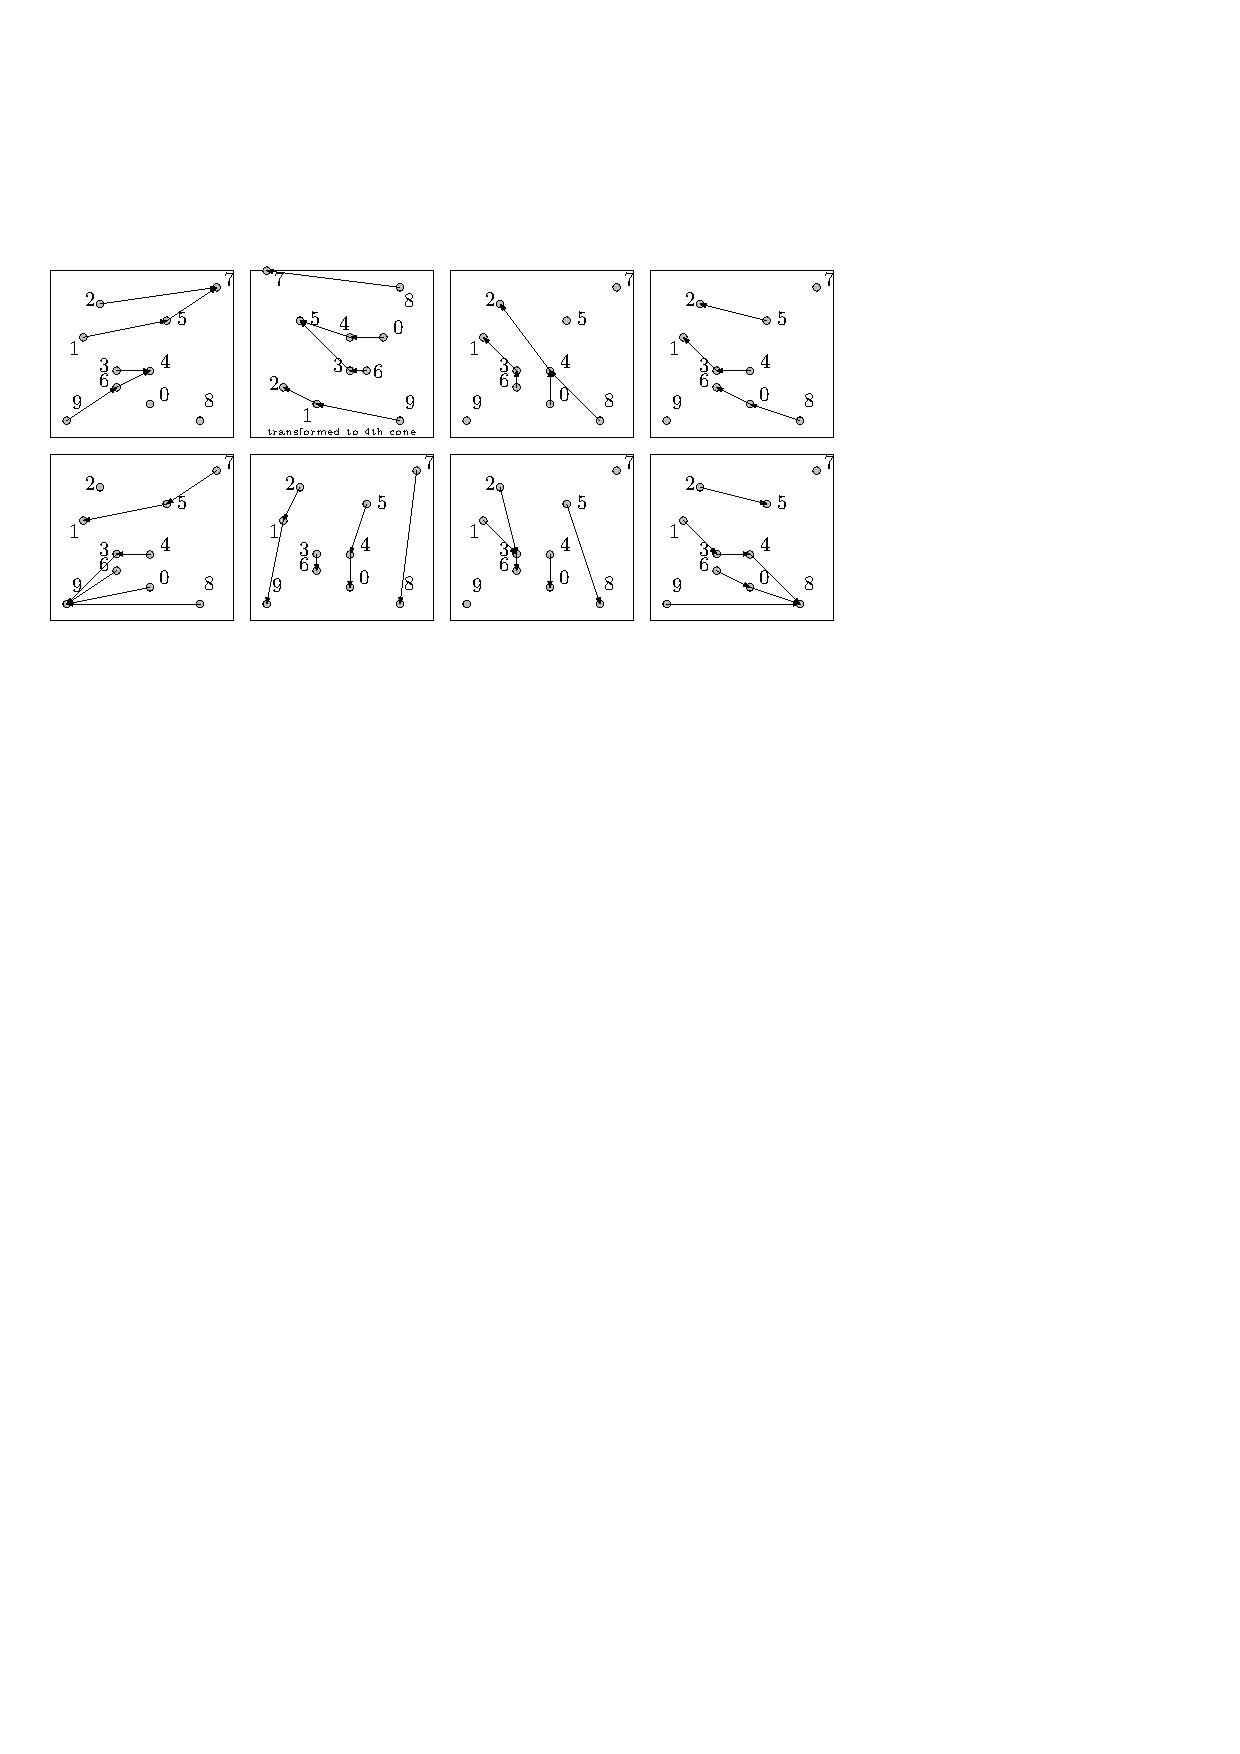
\includegraphics[width=\textwidth]{Figures/NearestNeighborinaCone.pdf}
\caption{L1 Nearest Neighbor in a Cone}
\label{fig:NearestNeighborinaCone}
\end{figure}

\subsubsection{L1 Nearest Neighbor in a Cone: $O(n \log n)$}
\begin{lstlisting}
Dictionary<int, int> N =
 NearestNeighbor.L1NearestNeighborInCone(P, ConeID);
\end{lstlisting}
Figure~\ref{fig:NearestNeighborinaCone} visually illustrates the output of the algorithm, when ConeID = $1,2,\ldots, 8$. Uses algorithm~\cite{?}.

\subsection{Array Search}

\subsubsection{Binary Search: $O(\log n)$}            \begin{lstlisting}
double[] A = {.251, .5468, .84245, .84245};            
int indexFound;
ArraySearch.BinarySearch(.251, A, out indexFound); 
\end{lstlisting}
\subsubsection{Binary Search Closest Neighbor: $O(\log n)$}           
\begin{lstlisting}
int l,r;
ArraySearch.BinarySearchClosest(1.2, A, out l, out r);
\end{lstlisting}



\newpage
\section{Data Structures}
\subsection{Segment Tree}
\begin{figure}[h]
\centering
\includegraphics[width=.5\textwidth]{Figures/segmenttree.pdf}
\caption{Segment Tree, Segment 4 is inserted in nodes 9, 18, 43}
\label{fig:NearestNeighborinaCone}
\end{figure}


\subsubsection{Construction: $O(n\log n)$}
\begin{lstlisting}
HInterval[] h = new HInterval[100];
//initialize h with unique ids
SegmentTree.Build(h);
\end{lstlisting}

\subsubsection{Get all Intersecting Segments $O(\log n)$}
\begin{lstlisting}
Point q = new Point(x,y);
List<HInterval> intervals =
 SegmentTree.GetAllIntersectingIntervals(q);
foreach (var interval in intervals) 
 Console.Write(interval.Id+",");
\end{lstlisting}

\subsubsection{Get the Segment Immediately Above $O(\log^2 n)$}
\begin{lstlisting}
Point q = new Point(x,y);
HInterval intv = 
 SegmentTree.GetImmediatelyAbove(q);
if (intv.Id > 0) Console.Write(intv.Id);
\end{lstlisting}






\end{document}

